\documentclass[border=6pt]{standalone}
\usepackage{ctex,amsmath,amssymb,tikz}
\usetikzlibrary{arrows.meta,positioning,patterns,calc,decorations.pathreplacing}
\begin{document}
% 图 13.1.2：曲线 y=f(x) 下的曲边梯形。
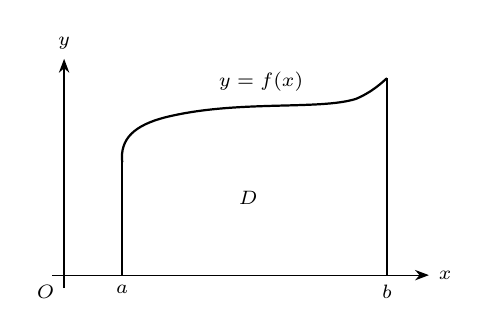
\begin{tikzpicture}[x=0.82cm,y=0.82cm,>=Stealth,baseline=(current bounding box.center)]
  \draw[->,line width=0.45pt] (-0.18,0) -- (5.65,0) node[right,font=\scriptsize] {$x$};
  \draw[->,line width=0.45pt] (0,-0.2) -- (0,3.35) node[above,font=\scriptsize] {$y$};
  \node[below left,font=\scriptsize] at (0,0) {$O$};
  \draw[line width=0.65pt] (0.9,0) -- (0.9,1.75);
  \draw[line width=0.65pt] (5.0,0) -- (5.0,3.05);
  \draw[line width=0.8pt]
    (0.9,1.75) .. controls (0.86,2.12) and (1.1,2.32) .. (1.55,2.44)
    .. controls (2.65,2.72) and (3.95,2.55) .. (4.52,2.73)
    .. controls (4.78,2.84) and (4.93,2.99) .. (5.0,3.05);
  \node[above,font=\scriptsize] at (3.05,2.69) {$y=f(x)$};
  \node[font=\scriptsize] at (2.85,1.2) {$D$};
  \node[below,font=\scriptsize] at (0.9,0) {$a$};
  \node[below,font=\scriptsize] at (5.0,0) {$b$};
\end{tikzpicture}

\end{document}